% !TEX root = main.tex
\section{Core Nebulas Rank}

Core Nebulas Rank se utiliza para medir las contribuciones de un usuario en referencia a la economía en su conjunto {\textbf{durante un periodo de tiempo dado}}.

El cálculo preciso es relativamente complicado, por lo que proponemos un algoritmo de aproximación para lograrlo. En este algoritmo de aproximación consideramos dos factores críticos: la \textit{acuñación} y la información de la posición de la cuenta en la red de transacciones. La siguiente sección de evaluación proporciona evidencia de la precisión de nuestro algoritmo de aproximación.

Utilizamos el historial de transacciones de la \textit{mainnet} durante un cierto período de tiempo como fuente de datos de Core Nebulas Rank.

Todas las transacciones durante un periodo de tiempo $[t_0-T,\ t_0]$ pueden ser especificadas como un conjunto:

\begin{align}
\Theta(t_0) = \{(s, t, w, \tau)\ |\ t_0 - T \le \tau \le t_0\ \land \ w > 0 \land s \neq t \}
\end{align}
\noindent Con base en $\Theta(t_0)$, podemos definir un grafo dirigido ponderado; el nodo hace referencia a la dirección de una cuenta, la arista que conecta el nodo $s$ con el nodo $d$ representa una transacción, la ponderación de la arista es $w$, el tiempo de la arista es $\tau$.

Para una cuenta $a \in \mathcal{A}$, el cálculo de Core Nebulas Rank $\mathcal{C}(a)$ se basa en $\Theta(t_0)$, que se puede representar como:
\begin{align}
\mathcal{C}(a) = \Omega(\beta(a)) \times{} \Psi(\gamma(a))
\label{eq:rank}
\end{align}
\noindent $\beta(a)$ es la media de la participación (\textit{stake}) de la cuenta $a$ en un periodo dado; $\gamma(a)$ es la valuación de ingresos y egresos de la cuenta $a$ en un periodo dado.

\whitepaper{A diferencia de los métodos de cálculo para Core Nebulas Rank definidos en el Libro Blanco Técnico de Nebulas \cite{Nebulas}, hemos hecho algunas actualizaciones que detallamos a continuación:\\
1. Dejamos de utilizar los montos de las transacciones $K$ más altas como factor de ponderación al construir los grafos de transacciones; \\
2. Ya no dependemos de la ponderación de los nodos de LeaderRank para obtener la importancia del nodo. \\
Primero, eliminamos los bucles de transacción antes de calcular la valuación de los ingresos y egresos $\beta$, de modo que resistir un ataque de transacciones cíclicas o en bucle. Al mismo tiempo aún tomamos en cuenta la fuerza de la arista. Para ciertos casos de grafos de topología homogénea, PageRank y otras funciones simétricas (como LeaderRank) han probado no ser capaces de resistir ataques Sybil \cite{cheng2005sybilproof}. En este libro amarillo ya no utilizamos la estrategia de valuación de tipo topológica; en su lugar, proponemos un cálculo asimétrico \refeq{eq:rank-param} que es efectivo para reducir las recompensas fingiendo los nodos de baja participación en \refsec{sec:function}.}

Abajo discutiremos tres problemas en \refeq{eq:rank}: Participación Media de Cuenta $\beta(a)$, Valuación de Ingresos y Egresos $\gamma(a)$, y la selección de la función $\Omega$ y $\Psi$.

\subsection{Participación Media de Cuenta $\beta(a)$}
En el periodo de tiempo de $[t_0-T, t_0]$, existen $n$ bloques en el sistema blockchain, marcados como:
\[
B_0, B_1, \dots, B_n
\]
\noindent $B_{i}$ se refiere al bloque padre de $B_{i+1}$. Para la cuenta $a \in \mathcal{A}$, el balance de la cuenta al final de cada bloque es:
\[
d^a_0, d^a_1, \dots, d^a_n
\]
Podemos obtener una nueva lista ordenando los elementos en orden ascendente:
\[
d^a_{(0)}, d^a_{(1)}, \dots, d^a_{(n)}
\]
\noindent donde $d^a_{(i)} < d^a_{(i+1)}, 0\le i \le {n-1}$, de esa forma, $\beta(a)$ se puede expresar como:
\begin{align}
\beta(a) = \left\{ \begin{array}{rcl}
{d^a_{(k)}} & \mbox{for} & n=2\times{}k, k=1, 2, 3, \ldots \\
{(d^a_{(k)} + d^a_{(k+1)})/2} & \mbox{for} & n=2\times{}k + 1, k=1, 2, 3, \ldots
\end{array}\right.
\end{align}
La participación media de la cuenta representa la acuñación de una cierta forma, lo que significa que la cuenta necesita mantener su participación por más de la mitad del periodo de tiempo.

\subsection{Valuación de Ingresos y Egresos $\gamma(a)$}
Considerando que un atacante podría incrementar su valuación de ingresos y egresos utilizando un ataque de bucle. Para evitar esta situación debemos remover el bucle de transacciones antes de calcular la valuación de ingresos y egresos para el grafo de transacciones. El bucle de transacciones es un ciclo dentro de un intervalo de tiempo.
Éste comienza y termina en el mismo nodo $v$, que es un conjunto de aristas en el grafo de transacciones. Un ciclo de transacciones puede ser denotado como $H(v)$:

\[
H(v) = \{(v, v_1, w_1, \tau_1), (v_1, v_2, w_2, \tau_2), \dots, (v_i, v_{i+1}, w_{i}, \tau_i), \dots, (v_n, v, w_{n+1}, \tau_{n+1})\}
\]
\noindent donde $\forall 1\le i \le n : \tau_i \le \tau_{i+1} $.
\noindent Como se muestra en \reffig{fig:loop}, hay un bucle de transacciones; nótese que la transacción $(v_1, v_2, 100, 5)$ no está incluida dentro de ese bucle.

\begin{figure}
\centering
  \begin{tikzpicture}
\pgfmathsetmacro{\XTD}{3.8}
\pgfmathsetmacro{\XMD}{1.2}
\pgfmathsetmacro{\YTD}{3.8}


\tikzset{
  node/.style={draw, circle, on grid, align=center, minimum height=2ex},
  thread/.style={draw, rectangle, on grid, align=center,color=gray!30,
  fill=gray!30,
  rounded corners,
  minimum height=3ex,fit=#1},
}

\node[node] (v) at (0, 0) {$v$};
\node[node] (v1) at (0, \YTD) {$v_1$};
\node[node] (v2) at (\XTD, \YTD) {$v_2$};
\node[node] (v3) at (\XTD, 0) {$v_3$};

\draw[->,>=stealth'] (v) to [out=135, in=225] node[left, midway] {$w=100$,$\tau=1$} (v1);
\draw[->,>=stealth'] (v1) to [out=45, in=135] node[above, midway] {$w=10$,$\tau=2$} (v2);
\draw[->,>=stealth'] (v1) to [out=315, in=225] node[below, midway] {$w=100$,$\tau=5$} (v2);
\draw[->,>=stealth'] (v2) to [out=315, in=45] node[right, midway] {$w=10$,$\tau=3$} (v3);
\draw[->,>=stealth'] (v3) to [out=225, in=315] node[below, midway] {$w=10$,$\tau=4$} (v);

\node at (2.5*\XTD, 0.5*\YTD) {
$\begin{aligned}
     H(v) = \{&(v, v1, 100, 1),\\
     &(v1, v2, 10, 2), \\
     &(v2, v3, 10, 3), \\
     &(v3, v, 10, 4) \}
  \end{aligned}$};
\end{tikzpicture}

\caption{loop\label{fig:loop}}
\end{figure}

\begin{figure}
\centering
\begin{tikzpicture}
\pgfmathsetmacro{\XTD}{3.8}
\pgfmathsetmacro{\XMD}{1.2}
\pgfmathsetmacro{\YTD}{3.8}


\tikzset{
  node/.style={draw, circle, on grid, align=center, minimum height=2ex},
  thread/.style={draw, rectangle, on grid, align=center,color=gray!30,
  fill=gray!30,
  rounded corners,
  minimum height=3ex,fit=#1},
}

\node[node] (v) at (0, 0) {$v$};
\node[node] (v1) at (0, \YTD) {$v_1$};
\node[node] (v2) at (\XTD, \YTD) {$v_2$};
\node[node] (v3) at (\XTD, 0) {$v_3$};
\draw[->,>=stealth'] (v) to [out=135, in=225] node[left, midway] {$w=90$,$\tau=1$} (v1);
\draw[->,>=stealth'] (v1) to [out=315, in=225] node[below, midway] {$w=100$,$\tau=5$} (v2);

\end{tikzpicture}
\caption{\reffig{fig:loop}去掉交易环后的交易图 \label{fig:no-loop}}
\end{figure}


Luego de determinar la existencia de estos bucles es necesario removerlos. Asumiendo que hay $n$ bucles en el sistema, y que éstos están listados por la secuencia que sigue:
\[
H^1(v_1), H^2(v_2), \dots, H^n(v_n)\]
\noindent La cantidad mínima de transacciones en $H^i(v_i)$ es $(s^i_m, t^i_m, w^i_m, \tau^i_m)$, y
\[
\forall (s^i, t^i, w^i, \tau^i) \in \mathcal{T} : w^i \ge w^i_m
\]
\noindent Así, por cada transacción en $H^i(v_i)$, necesitamos reducir el monto mínimo de transacción $w^i_m$ de forma acorde y eliminar esta transacción si el monto de la última transacción es 0:
\[
\mathcal{E}((s, t, w, \tau), w_m) = \left\{ \begin{array}{rcl}
(s, t, w-w_m, \tau) & \mbox{if} & w \ne w_m \\
\phi & \mbox{if} & w = w_m
\end{array}\right.
\]
\begin{align}
\Theta^{\prime}(t_0)=\Theta(t_0)-H^i(v) \cup \{\mathcal{E}(t), t\in H^i(v_i)\} \quad i = 1, 2,\dots, n
\end{align}
\noindent La \reffig{fig:no-loop} nos muestra el grafo de la transacción sin bucles luego de remover el bucle de transacciones en \reffig{fig:loop}.


Fijamos el monto de ingreso al nodo $v$ como $p(v)$, entonces
\begin{align}
\label{eq:dgr_func}
p(v) = \sum_{(s_i, v, w_i, \tau_i) \in \Theta^{\prime}(t_0)}{w_i}
\end{align}
\noindent Similarmente, fijamos el monto de egreso del nodo $v$, que es
\begin{align}
q(v) = \sum_{(v, t_i, w_i, \tau_i) \in \Theta^{\prime}(t_0)}{w_i}
\end{align}
\noindent En este caso,
para el nodo $v$, su valuación de ingresos y egresos $\gamma(v)$ es

\begin{align}
\mathcal{G}(v) = (p(v) + q(v)) \cdot e^{-2\sin^2{(\frac{\pi}{4} - \arctan\frac{q(v)}{p(v)})}}
\end{align}
\begin{align}
\gamma(v) = (\frac{\theta\cdot \mathcal{G}(v)}{\mathcal{G}(v) + \mu})^{\lambda}
\end{align}
\noindent donde $\theta, \mu, \lambda$ son los parámetros a ser determinados.


Y la \reffig{fig-surf} muestra la curva de la \refeq{eq:dgr_func}.
\begin{figure}
  \centering
  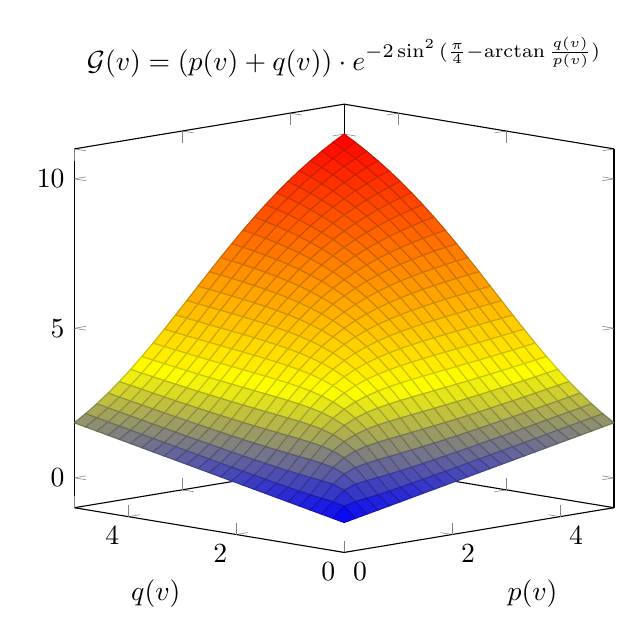
\begin{tikzpicture}[
    declare function={tf(\x)=(pi/4-rad(atan(\x)));},
    declare function={func(\x,\y)=sin(tf(\y/\x)*180/pi);}
]
\begin{axis}[
    view={315}{10},
    title={$
\mathcal{G}(v) = (p(v) + q(v)) \cdot e^{-2\sin^2{(\frac{\pi}{4} -
\arctan\frac{q(v)}{p(v)})}}$},
    xlabel=$p(v)$,
    ylabel=$q(v)$,
]

\addplot3 [
        surf,
        domain=0:5,
        domain y=0:5,
    ] {(x+y)*exp((-2)*(func(x,y))^2)};
\end{axis}
\end{tikzpicture}

\caption{La curva de la función de valuación de ingresos y egresos \label{fig-surf}}
\end{figure}

\subsection{Función Wilbur \label{sec:function}}
Es extremadamente complicado calcular Core Nebulas Rank si consideramos los distintos usos posibles y sus propiedades. Sin embargo, es posible proveer una función más general para Nebulas Rank.

Definimos la función de cálculo de Core Nebulas Rank como \(f(x)\), a saber \emph{Función Wilbur}\footnote{El nombre \emph{Ataque Sybil} deriva de una serie de TV de los años 1970 llamada Sybil, en la que una mujer joven es diagnosticada con un trastorno de personalidades múltiples y recibe su tratamiento con la doctora Cornelia Wilbur.}, donde \(x\) es el factor de Core Nebulas Rank; éste puede ser una cuenta de participación, una acuñación la valuación de ingresos y egresos. $f(x)$ satisface dos propiedades:

\begin{property}
\label{prop:one}
Para dos variables cualesquiera $x_1$ y $x_2$, ambas mayores que $0$, la suma de las dos funciones es menor que la función de suma de las dos variables.
\end{property}

\begin{align}
f(x_1+x_2)>f(x_1)+f(x_2) \quad x_1>0,x_2>0
\end{align}

\begin{property}
\label{prop:two}
Para dos variables cualesquiera $x_1$ y $x_2$ cuyos valores son infinitos, la suma de las dos funciones es aproximadamente igual a la función de la suma de las dos variables.
\end{property}

\begin{align}
\lim\limits_{x_1 \to \infty, x_2\to \infty} f(x_1+x_2) = f(x_1) + f(x_2)\quad x_1>0, x_2>0
\end{align}

Las dos propiedades descritas arriba aseguran que, bajo determinadas conductas de transacción, el beneficio de dividir la participación en cuentas más pequeñas es comparativamente menor que mantenerlo dentro de una sola cuenta. Al mismo tiempo, cuando la participación es lo suficientemente grande, el costo de dividirla en cuentas más pequeñas puede ser ignorado.

Existe más de una función que satisface las dos propiedades descritas arriba. Aquí proveemos una función sucinta; la curva de esta función se muestra en \reffig{fig-nr}.
\begin{align}
f(x) = x/(1 + e^{a + b\cdot x}) \quad a>1,b<0
\end{align}
\noindent {La prueba detallada de la función se da en el anexo ~\ref{sec:appendix_proof}}

\begin{figure}
\centering
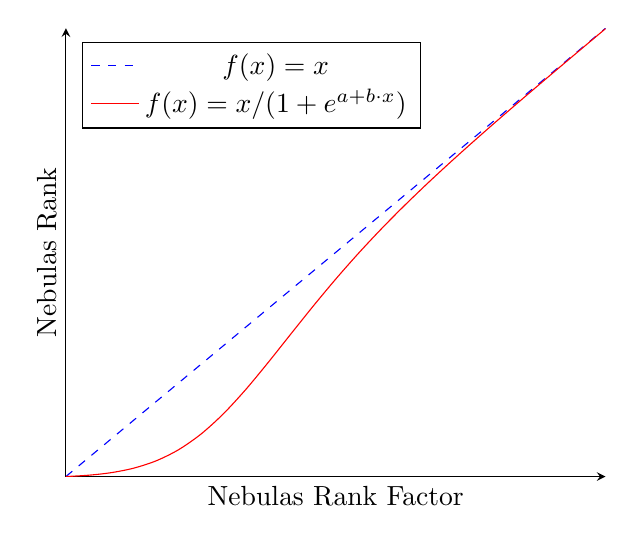
\begin{tikzpicture}[
    declare function={func(\x,\mu) = (\x / (1 + exp(\mu-\x)));},
    declare function={linefunc(\x) = \x;}
]
\begin{axis}[
    axis lines=left,
    enlargelimits=upper,
ticks=none,axis x line=bottom,axis y line=left,xlabel={Nebulas Rank Factor},
  ylabel={Nebulas Rank},
      legend pos=north west,
legend style={fill=none}
]
\addplot [dashed, domain=0:10, blue] {linefunc(x)};
\addplot [smooth, domain=0:10, red] {func(x,3)};
\addlegendentry{$f(x)=x$}
\addlegendentry{$f(x)=x/(1 + e^{a + b\cdot x})$}
\end{axis}
\end{tikzpicture}
\caption{La curva de la función Nebulas Rank \label{fig-nr}}
\end{figure}


\vspace{2em}
En síntesis, \refeq{eq:rank} se puede expresar de este manera:

\begin{align}
\label{eq:rank-param}
\mathcal{C}(v) =  \frac{\beta(v)}{1+e^{a + b \cdot \beta(v)}} \cdot \frac{\gamma(v)}{1+e^{c + d \cdot \gamma(v)}}
\end{align}
\noindent donde $a, b, c, d$ son parámetros a ser determinados.


Con el fin de verificar la efectividad de la función, calculamos el valor Core Nebulas Rank para todas las cuentas registradas en el blockchain Ethereum durante un período dado. Recogimos todos los registros de transacciones desde el primero de mayo de 2017 hasta el 30 de junio de ese mismo año (altura de bloque: desde 3629091 hasta 3955158), en suma, también recogimos el valor promedio diario de ETH (en dólares) y los volúmenes de transacciones \cite{coinmarketcap}.

La \reffig{fig-eth-simu} muestra la tendencia entre la capitalización del mercado ETH y el valor
Core Nebulas Rank para Ethereum, donde la línea sólida negra indica
la capitalización de mercado para Ethereum (en dólares), mientras la línea sólida roja representa
la suma de todas las cuentas Core Nebulas Rank basadas en \refeq{eq:rank-param}.

Podemos ver que Core Nebulas Rank refleja los cambios en la capitalización de mercado de Ethereum de forma precisa. El coeficiente de correlación es de 0.84427, mientras que $p$
(valor p, o significancia) es de $4.48\times{}10^{-17}<0.001$. Esto significa que \refeq{eq:rank} ilustra el éxito en describir las contribuciones de los usuarios al sistema económico en el blockchain, lo que demuestra tanto la validez y la precisión de Core Nebulas Rank.


\begin{figure}
\centering
\begin{tikzpicture}
  \begin{axis}[
  axis y line*=left,
  axis x line=none,
%ticks=none,
ylabel={Capitalización de mercado de Ethereum (en dólares) },
%xtick={0,10,20,30,40,50,60},
%xlabel={Time(Day)}
legend style={fill=none}
    ]
\addplot[smooth, mark=., color=red] table [x=day, y=nr, col sep=comma]
    {../common/eth_simu.csv};
\label{plot_one}

\end{axis}
  \begin{axis}[
%ticks=none,
legend pos=north west,
%ylabel={Nebulas Rank},
xlabel={Time (day) },
xtick={0,10,20,30,40,50,60},
ytick={1,2},
axis y line*=right,
legend style={fill=none}
    ]
    \addlegendimage{/pgfplots/refstyle=plot_one}\addlegendentry{Nebulas Rank}

    \addplot[smooth, mark=x] table [x=day, y=cap, col sep=comma]
    {../common/eth_simu.csv};
    \label{plot_two}
      \addlegendentry{Cap. Mercado de ETH}
\end{axis}

\end{tikzpicture}
\caption{La capitalización de mercado y el valor Core Nebulas Rank de Ethereum}
\label{fig-eth-simu}
\end{figure}